\documentclass[final]{beamer}
\usepackage{eulervm,verbatim}          
\usepackage[scaled]{helvet}
\usepackage[most]{tcolorbox}
\setbeamercolor{frametitle}{fg=black,bg=white} % Colors of the block titles
\setbeamertemplate{caption}{\raggedright\insertcaption\par}
\setbeamertemplate{caption}{\raggedright\insertcaption\par}
\definecolor{darkcerulean}{rgb}{0.03, 0.27, 0.49}
\newcommand{\citesmall}[1]{[{\color{darkcerulean}\begin{small} \textbf{#1} \end{small}}]}
\setbeamertemplate{footline}[frame number]
\DeclareMathOperator*{\argmin}{arg\,min}
\usepackage{graphicx}  % Required for including images
\usepackage{bbm}
\usepackage{booktabs} % Top and bottom rules for tables
\definecolor{burgundy}{rgb}{0.5, 0.0, 0.13}
\newcommand{\highlight}[1]{{\color{burgundy} \textbf{#1}}}
\usepackage{hyperref}
\hypersetup{
    colorlinks=true,
    linkcolor=blue,
    filecolor=magenta,      
    urlcolor=magenta,
    pdftitle={CSE6740-Lecture 3},
    pdfauthor={Nisha Chandramoorthy},
    pdflang={en-US}
}



%----------------------------------------------------------------------------------------
%	TITLE SECTION 
%----------------------------------------------------------------------------------------
\title{\begin{huge}{CSE 6740 A/ISyE 6740: Computational Data Analysis: Introductory lecture}\end{huge}} % Poster title


\author{Nisha Chandramoorthy} % Author(s)


%----------------------------------------------------------------------------------------

\begin{document}

\frame{\titlepage}

%----------------------------------------------------------------------------------------
%	OBJECTIVES
%----------------------------------------------------------------------------------------
\begin{frame}{Last time}
\begin{itemize}
	\item Least squares regression
	\pause 
	\item Gauss-Markov theorem
	\pause 
	\item Ridge regression, optimization and geometric perspectives
	\pause
	\item Shrinkage
\end{itemize}
\end{frame}
\begin{frame}{Today}
\begin{itemize}
	\item Shrinkage by ridge regression
	\pause
	\item Geometric view of LASSO
	\pause
	\item Generalization of LASSO 
	\pause 
	\item $\ell^0$ regularization and compressed sensing
	\pause
\end{itemize}
\end{frame}
\begin{frame}
	\begin{itemize}
	\item Online linear regression algorithms
	\pause 
	\item Classification ERM
	\pause
	\item Perceptron algorithm
	\pause
	\item Convergence proof of perceptron algorithm 
	\end{itemize}
\end{frame}
\begin{frame}{Compression by LASSO}
	\begin{figure}
		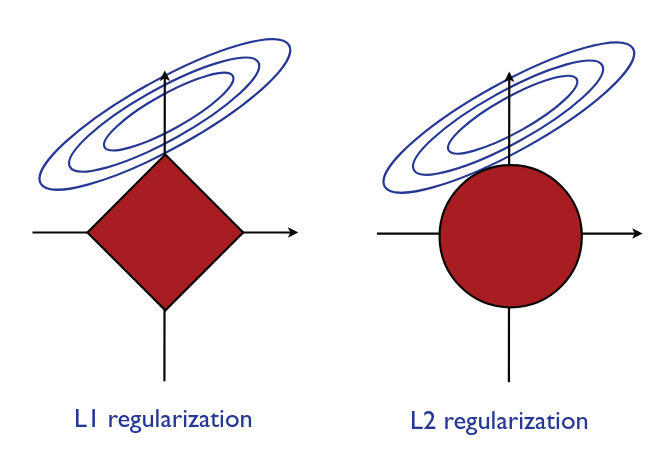
\includegraphics[width=\textwidth]{lasso.png}
	\end{figure}
\end{frame}


\end{document}
